
% ===========================================================================
% Title:
% ---------------------------------------------------------------------------
% to create Type I fonts type "dvips -P cmz -t letter <filename>"
% ===========================================================================
\documentclass[11pt]{article}       %--- LATEX 2e base
\usepackage{latexsym}               %--- LATEX 2e base
%---------------- Wide format -----------------------------------------------
\textwidth=6in \textheight=9in \oddsidemargin=0.25in
\evensidemargin=0.25in \topmargin=-0.5in
%--------------- Def., Theorem, Proof, etc. ---------------------------------
\newtheorem{definition}{Definition}
\newtheorem{theorem}{Theorem}
\newtheorem{lemma}{Lemma}
\newtheorem{corollary}{Corollary}
\newtheorem{property}{Property}
\newtheorem{observation}{Observation}
\newtheorem{fact}{Fact}
\newenvironment{proof}           {\noindent{\bf Proof.} }%
                                 {\null\hfill$\Box$\par\medskip}
%--------------- Algorithm --------------------------------------------------
\newtheorem{algX}{Algorithm}
\newenvironment{algorithm}       {\begin{algX}\begin{em}}%
                                 {\par\noindent --- End of Algorithm ---
                                 \end{em}\end{algX}}
\newcommand{\step}[2]            {\begin{list}{}
                                  {  \setlength{\topsep}{0cm}
                                     \setlength{\partopsep}{0cm}
                                     \setlength{\leftmargin}{0.8cm}
                                     \setlength{\labelwidth}{0.7cm}
                                     \setlength{\labelsep}{0.1cm}    }
                                  \item[#1]#2    \end{list}}
                                 % usage: \begin{algorithm} \label{xyz}
                                 %        ... \step{(1)}{...} ...
                                 %        \end{algorithm}
%--------------- Figures ----------------------------------------------------
\usepackage{graphicx}

\newcommand{\includeFig}[3]      {\begin{figure}[htb] \begin{center}
                                 \includegraphics
                                 [width=4in,keepaspectratio] %comment this line to disable scaling
                                 {#2}\caption{\label{#1}#3} \end{center} \end{figure}}
                                 % usage: \includeFig{label}{file}{caption}
%--------------- Additiona packages -----------------------------------------
\usepackage{url}
\usepackage{tikz}
\usetikzlibrary{positioning}
\tikzset{font=\scriptsize}
% ===========================================================================
\begin{document}
% ===========================================================================

% ############################################################################
% Title
% ############################################################################

\title{LITERATURE REVIEW: XRT 0.1.0 - A Language-Agnostic Map-Reduce Runtime for
Shared-Memory Systems}


% ############################################################################
% Author(s) (no blank lines !)
\author{
% ############################################################################
Erik Selin\\
School of Information Technology and Engineering\\
University of Ottawa\\
Ottawa, Canada K1N 6N5 \\
{\em erik.selin@gmail.com}
% ############################################################################
} % end-authors
% ############################################################################

\maketitle

% ############################################################################
\section{Introduction} \label{intro}
% ############################################################################

% start from parallel computing in general and lead to your particular topic
% It may provide background or history
% work has been done on the topic

Map-reduce is a restrictive programming model introduced in 2004 by Google
\cite{dean2004mapreduce} and later popularized by the open-source Apache project
Hadoop MapReduce developed by a team at Yahoo! \cite{Hadoop}. At a high level,
map-reduce enables developers to write efficient and highly parallelizable data
processing jobs without having to deal with the complexities of parallel
programming. Following the initial success of Hadoop MapReduce and the growing
need for processing of so called big data multiple map-reduce runtimes have been
developed for various environments. Map-reduce is becoming particularly
interesting for shared-memory systems as core counts and memory availability is
steadily increasing while cost is going down.

% The introduction explains the focus and establishes the importance of subject
% identifies any controversies within the field
% any recent research which has raised questions

Multiple map-reduce runtimes have been developed for shared-memory systems but
the focus of these systems is almost entirely to compete for best in-memory
benchmarks while sacrificing usability, simplicity and cross platform
compatibility \cite{Phoenix} \cite{CilkMR} \cite{TODO...}. Processing of data
that does not fit in system memory is rarely if ever discussed in the current
shared-memory map-reduce runtimes. In addition all of these runtimes forces the
programmer to implement data processing jobs in C++ which is simply not an
option for most engineering teams. Attempts have been made to bring a more
flexible map-reduce runtime through the Hadoop Streaming project
\cite{HadoopStreaming} but since it is built upon Hadoop MapReduce it suffers
from major performance issues \cite{...}. Attempts have been made to speed-up
Hadoop MapReduce for shared-memory systems \cite{...} and to add support for
languages to Hadoop MapReduce \cite{...} \cite{...} \cite{...}. Unfortunately
none of these projects have yielded a performant language-agnostic shared-memory
runtime.

% Introduce your project topic
% suggest how the review findings will lead to the research
% Describe what you intend to achieve in your project
% It concludes with a purpose or thesis statement.

XRT is a response to these perceived shortcomings in the shared-memory
map-reduce community. It is a map-reduce runtime built from the ground up for
high performance on shared-memory systems while offering a completely
language-agnostic API. XRT is memory-first but disk-aware and uses the streaming
model from Hadoop Streaming \cite{} but with a runtime inspired by Phoenix,
CilkMR and other shared-memory map-reduce runtimes \cite{} \cite{}.

% ############################################################################
\section{Literature Review} \label{litrev}
% ############################################################################

\subsection{The map-reduce programing model}

\begin{figure}[h]
  \centering
  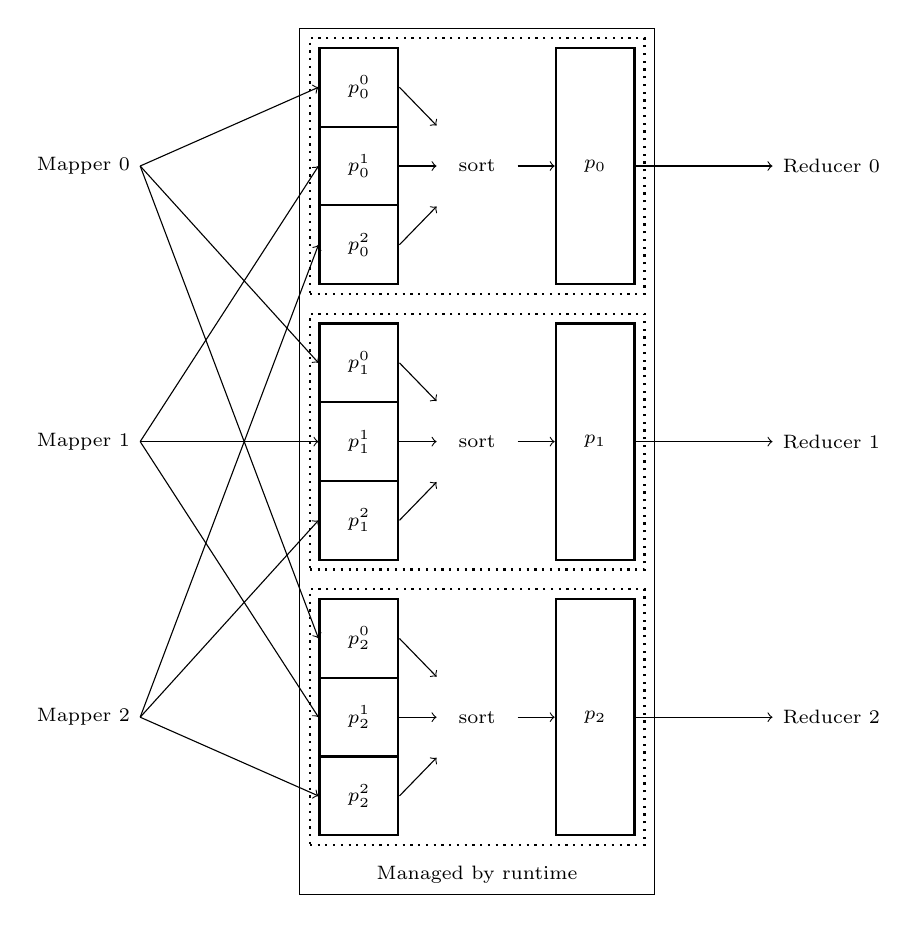
\begin{tikzpicture}[every node/.style={minimum height={1cm},minimum width={1cm},thick}]
      \node (M2) at (0,1.5) {Mapper 2};
      \node (M1) at (0,5) {Mapper 1};
      \node (M0) at (0,8.5) {Mapper 0};

      \node[draw] (P20) at (3.5,2.5) { $p_2^0$ };
      \node[draw] (P21) at (3.5,1.5) { $p_2^1$ };
      \node[draw] (P22) at (3.5,0.5) { $p_2^2$ };
      \node (S2) at (5,1.5) {sort};
      \node[draw,minimum height={3cm}] (B2) at (6.5, 1.5) { $p_2$ };
      \node[draw,dotted,minimum height={3.25cm},minimum width={4.25cm}] (P2) at (5,1.5) {};

      \node[draw] (P10) at (3.5,6) { $p_1^0$ };
      \node[draw] (P11) at (3.5,5) { $p_1^1$ };
      \node[draw] (P12) at (3.5,4) { $p_1^2$ };
      \node (S1) at (5,5) {sort};
      \node[draw,minimum height={3cm}] (B1) at (6.5, 5) { $p_1$ };
      \node[draw,dotted,minimum height={3.25cm},minimum width={4.25cm}] (P1) at (5,5) {};

      \node[draw] (P00) at (3.5,9.5) { $p_0^0$ };
      \node[draw] (P01) at (3.5,8.5) { $p_0^1$ };
      \node[draw] (P02) at (3.5,7.5) { $p_0^2$ };
      \node (S0) at (5,8.5) {sort};
      \node[draw,minimum height={3cm}] (B0) at (6.5, 8.5) { $p_0$ };
      \node[draw,dotted,minimum height={3.25cm},minimum width={4.25cm}] (P0) at (5,8.5) {};

      \node (R2) at (9.5,1.5) {Reducer 2};
      \node (R1) at (9.5,5) {Reducer 1};
      \node (R0) at (9.5,8.5) {Reducer 0};

      \node at (5,-0.5) {Managed by runtime};
      \node[draw,thin,minimum height={11cm},minimum width={4.5cm}] (P) at (5,4.75) {};

      \path [->](M0.east) edge node {} (P00.west);
      \path [->](M0.east) edge node {} (P10.west);
      \path [->](M0.east) edge node {} (P20.west);
      \path [->](M1.east) edge node {} (P01.west);
      \path [->](M1.east) edge node {} (P11.west);
      \path [->](M1.east) edge node {} (P21.west);
      \path [->](M2.east) edge node {} (P02.west);
      \path [->](M2.east) edge node {} (P12.west);
      \path [->](M2.east) edge node {} (P22.west);

      \path [->](P00.east) edge node {} (S0.north west);
      \path [->](P01.east) edge node {} (S0.west);
      \path [->](P02.east) edge node {} (S0.south west);
      \path [->](P10.east) edge node {} (S1.north west);
      \path [->](P11.east) edge node {} (S1.west);
      \path [->](P12.east) edge node {} (S1.south west);
      \path [->](P20.east) edge node {} (S2.north west);
      \path [->](P21.east) edge node {} (S2.west);
      \path [->](P22.east) edge node {} (S2.south west);

      \path [->](S0.east) edge node {} (B0.west);
      \path [->](S1.east) edge node {} (B1.west);
      \path [->](S2.east) edge node {} (B2.west);

      \path [->](B0.east) edge node {} (R0.west);
      \path [->](B1.east) edge node {} (R1.west);
      \path [->](B2.east) edge node {} (R2.west);
  \end{tikzpicture}
  \caption{In map-reduce runtimes the programmer provides the mapper and reducer code while input, output, execution of mapper code, execution of reducer code, shuffling and sorting is handled by the runtime.}
\end{figure}


\subsection{Map-reduce on GPUs, FPGA and Coprocessors}

\subsection{Map-reduce on shared-memory runtimes}

\begin{figure}[h]
  \centering
  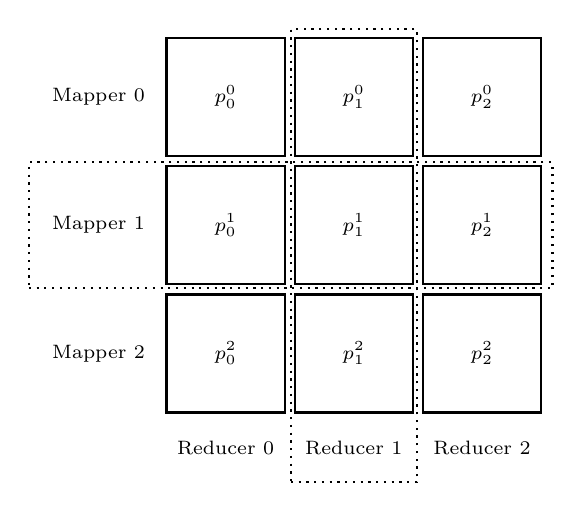
\begin{tikzpicture}[every node/.style={minimum height={1.5cm},minimum width={1.5cm},thick}]
    \matrix[row sep=1mm, column sep=1mm] (m)
    {
      \node { Mapper 0 }; & \node[draw] { $p_0^0$ }; & \node[draw] (c1) { $p_1^0$ }; & \node[draw] { $p_2^0$}; \\
      \node (r1) { Mapper 1 }; & \node[draw] { $p_0^1$ }; & \node[draw] { $p_1^1$ }; & \node[draw] { $p_2^1$ }; \\
      \node { Mapper 2 }; & \node[draw] (node0) { $p_0^2$}; & \node[draw] (node1) { $p_1^2$ }; & \node[draw] (node2) { $p_2^2$ }; \\
    };

    \node[below=1.75cm of node0.north,minimum height=0cm] {Reducer 0};
    \node[below=1.75cm of node1.north,minimum height=0cm] {Reducer 1};
    \node[below=1.75cm of node2.north,minimum height=0cm] {Reducer 2};

    \node[below=-1.1mm of c1.north,draw,dotted,minimum height=5.75cm,minimum width=1.6cm] {};
    \node[below right=-0.5mm and -0.9cm of r1.north,draw,dotted,minimum height=1.6cm,minimum width=6.65cm] {};
  \end{tikzpicture}
  \caption{In shared-memory map-reduce systems memory is usually split into a matrix. Mappers are given access to a single row and partitions data into the entries of that row. Reducers are given access to a single column where all entries represents the same partition.}
\end{figure}

XRT is a response to these perceived shortcomings in the shared-memory
map-reduce community. It is a map-reduce runtime built from the ground up for
high performance on shared-memory systems while offering a completely
language-agnostic API. XRT is memory-first but disk-aware and uses the streaming
model from Hadoop Streaming \cite{} but with a runtime inspired by Phoenix,
CilkMR and other shared-memory map-reduce runtimes \cite{} \cite{}.

XRT is a response to these perceived shortcomings in the shared-memory
map-reduce community. It is a map-reduce runtime built from the ground up for
high performance on shared-memory systems while offering a completely
language-agnostic API. XRT is memory-first but disk-aware and uses the streaming
model from Hadoop Streaming \cite{} but with a runtime inspired by Phoenix,
CilkMR and other shared-memory map-reduce runtimes \cite{} \cite{}.

\subsection{Language-agnostic map-reduce}

\subsection{Data over standard streams}

% ############################################################################
% Bibliography
% ############################################################################
\bibliographystyle{plain}
\bibliography{bibliography}     %loads bibliography.bib

% ============================================================================
\end{document}
% ============================================================================
